% Options for packages loaded elsewhere
\PassOptionsToPackage{unicode}{hyperref}
\PassOptionsToPackage{hyphens}{url}
%
\documentclass[
  11pt,
]{article}
\usepackage{lmodern}
\usepackage{amssymb,amsmath}
\usepackage{ifxetex,ifluatex}
\ifnum 0\ifxetex 1\fi\ifluatex 1\fi=0 % if pdftex
  \usepackage[T1]{fontenc}
  \usepackage[utf8]{inputenc}
  \usepackage{textcomp} % provide euro and other symbols
\else % if luatex or xetex
  \usepackage{unicode-math}
  \defaultfontfeatures{Scale=MatchLowercase}
  \defaultfontfeatures[\rmfamily]{Ligatures=TeX,Scale=1}
\fi
% Use upquote if available, for straight quotes in verbatim environments
\IfFileExists{upquote.sty}{\usepackage{upquote}}{}
\IfFileExists{microtype.sty}{% use microtype if available
  \usepackage[]{microtype}
  \UseMicrotypeSet[protrusion]{basicmath} % disable protrusion for tt fonts
}{}
\makeatletter
\@ifundefined{KOMAClassName}{% if non-KOMA class
  \IfFileExists{parskip.sty}{%
    \usepackage{parskip}
  }{% else
    \setlength{\parindent}{0pt}
    \setlength{\parskip}{6pt plus 2pt minus 1pt}}
}{% if KOMA class
  \KOMAoptions{parskip=half}}
\makeatother
\usepackage{xcolor}
\IfFileExists{xurl.sty}{\usepackage{xurl}}{} % add URL line breaks if available
\IfFileExists{bookmark.sty}{\usepackage{bookmark}}{\usepackage{hyperref}}
\hypersetup{
  pdftitle={Tractament vs.~Control},
  pdfauthor={Aida Fernandez, 1497182},
  hidelinks,
  pdfcreator={LaTeX via pandoc}}
\urlstyle{same} % disable monospaced font for URLs
\usepackage{graphicx,grffile}
\makeatletter
\def\maxwidth{\ifdim\Gin@nat@width>\linewidth\linewidth\else\Gin@nat@width\fi}
\def\maxheight{\ifdim\Gin@nat@height>\textheight\textheight\else\Gin@nat@height\fi}
\makeatother
% Scale images if necessary, so that they will not overflow the page
% margins by default, and it is still possible to overwrite the defaults
% using explicit options in \includegraphics[width, height, ...]{}
\setkeys{Gin}{width=\maxwidth,height=\maxheight,keepaspectratio}
% Set default figure placement to htbp
\makeatletter
\def\fps@figure{htbp}
\makeatother
\setlength{\emergencystretch}{3em} % prevent overfull lines
\providecommand{\tightlist}{%
  \setlength{\itemsep}{0pt}\setlength{\parskip}{0pt}}
\setcounter{secnumdepth}{-\maxdimen} % remove section numbering

\title{Tractament vs.~Control}
\author{Aida Fernandez, 1497182}
\date{}

\begin{document}
\maketitle

\hypertarget{gestiuxf3-de-les-dades}{%
\subsection{Gestió de les dades}\label{gestiuxf3-de-les-dades}}

Llegim les dades \emph{pesosIndividuales.xlsx}

Posem les variables ``Box'' i ``Treat'' com a factors.

\begin{verbatim}
##  [1] "1"  "2"  "3"  "4"  "5"  "6"  "7"  "8"  "9"  "10" "11" "12" "13" "14" "15"
## [16] "16" "17" "18" "19" "20" "21" "22" "23" "24" "25" "26" "27" "28" "29" "30"
## [31] "31" "32" "33" "34" "35" "36" "37" "38" "39" "40" "41" "42" "43" "44" "45"
## [46] "46" "47" "48" "49" "50" "51" "52" "53" "54" "55" "56" "57" "58" "59" "60"
## [61] "61" "62" "63" "64" "65" "66" "67" "68" "69" "70" "71" "72" "73" "74" "75"
## [76] "76" "77" "78" "79" "80"
\end{verbatim}

\begin{verbatim}
## [1] "1" "2" "3" "4" "5" "6" "7" "8"
\end{verbatim}

Creem les següents varibles d'interès.

Guany de pes: \[BW_{41-28} = BW_{41} - BW_{28}\]

Index de l'increment de pes:
\[Index_{41-28} = 100*\cfrac{BW_{41}}{BW_{28}}\]

Taxa de l'increment de pes:
\[Taxa_{41-28} = 100*\cfrac{BW_{41}-BW_{28}}{BW_{28}}\]

\hypertarget{tractament-de-les-dades-faltants}{%
\subsubsection{Tractament de les dades
faltants}\label{tractament-de-les-dades-faltants}}

\hypertarget{eliminaciuxf3-de-les-dades-faltants}{%
\paragraph{Eliminació de les dades
faltants}\label{eliminaciuxf3-de-les-dades-faltants}}

Si concluim en que la distribució de les dades faltants es pot
considerar aleatòria i que n'hi ha poques podem omitir aquestes dades i
treure-les de la base de dades sabent que no esbiaixaràn l'anàlisi.
Encara que cal tenir en compte que hi haurà una petita pèrdua
d'informació.

\hypertarget{comparaciuxf3-gruxe0fica}{%
\subsection{Comparació gràfica}\label{comparaciuxf3-gruxe0fica}}

Package per a fer layouts de ggplot2

Amb les següents llibraries podrem obtenir ggplots d'una manera
considerablement senzilla.

Funció per a simplificar l'obtenció dels histogrames per a comparar
tractaments. Els arguments de la funció són:

\begin{itemize}
\item
  ``BD'' la base de dades.
\item
  ``Trac1'' i ``Tract2'' són els tractaments a comparar.
\item
  ``TipusGraf'' si és 1 representem els histogrames solapant-se al
  mateix eix de les y, si val 2 representarem els histogrames un a sobre
  de l'altre pero en diferents eix y.
\item
  ``NombreBins'' és el nombre de ``caixes'' en que estarà dividit
  l'histograma de cadascún dels tractaments, el valor predeterminat és
  10.
\item
  ``var'' és la variable sobre la que es faràn els histogrames.
\end{itemize}

Histogrames de les noves variables:
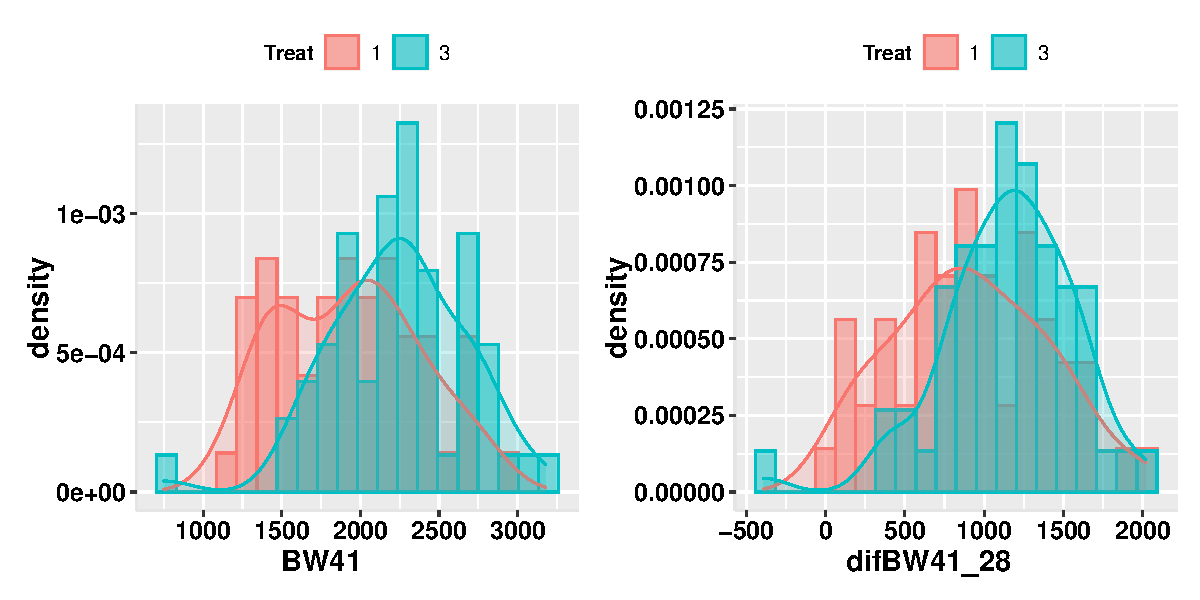
\includegraphics{def_files/figure-latex/unnamed-chunk-10-1.pdf}
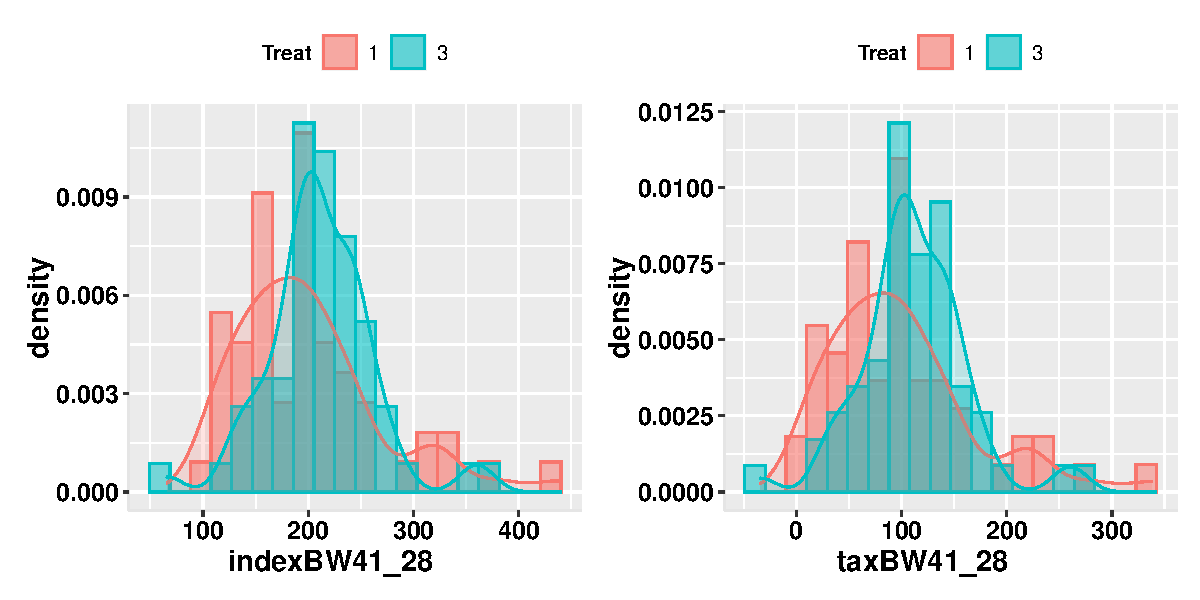
\includegraphics{def_files/figure-latex/unnamed-chunk-10-2.pdf}

\hypertarget{comparaciuxf3-de-tots-els-tractaments-amb-el-control}{%
\subsubsection{Comparació de tots els tractaments amb el
control}\label{comparaciuxf3-de-tots-els-tractaments-amb-el-control}}

\hypertarget{variable-bw41}{%
\paragraph{\texorpdfstring{Variable
\emph{BW41}}{Variable BW41}}\label{variable-bw41}}

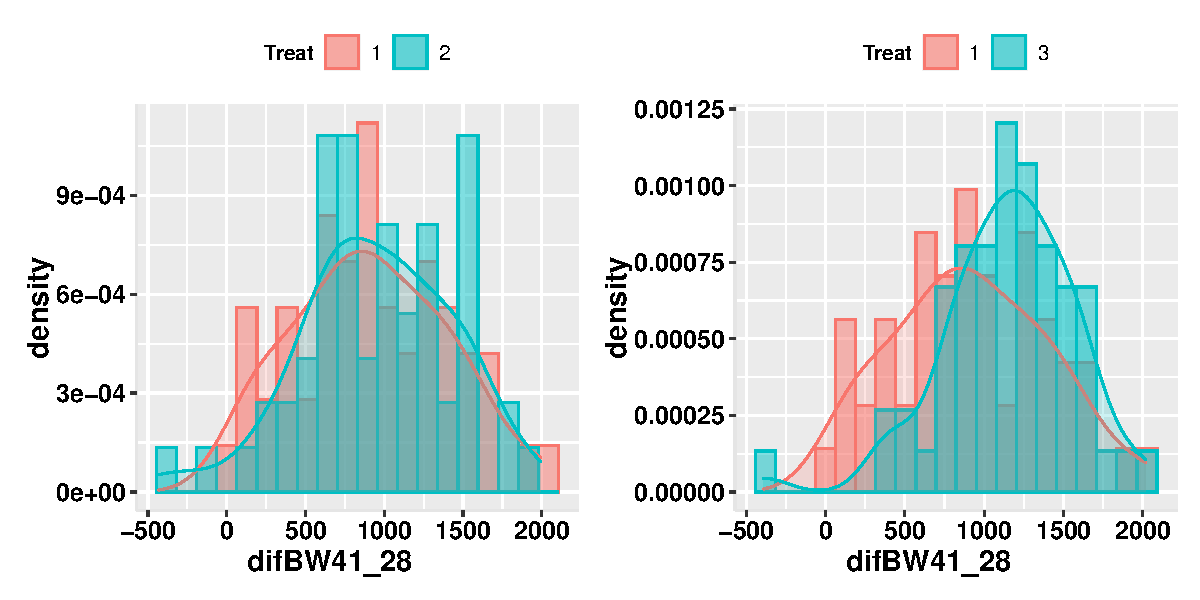
\includegraphics{def_files/figure-latex/unnamed-chunk-12-1.pdf}
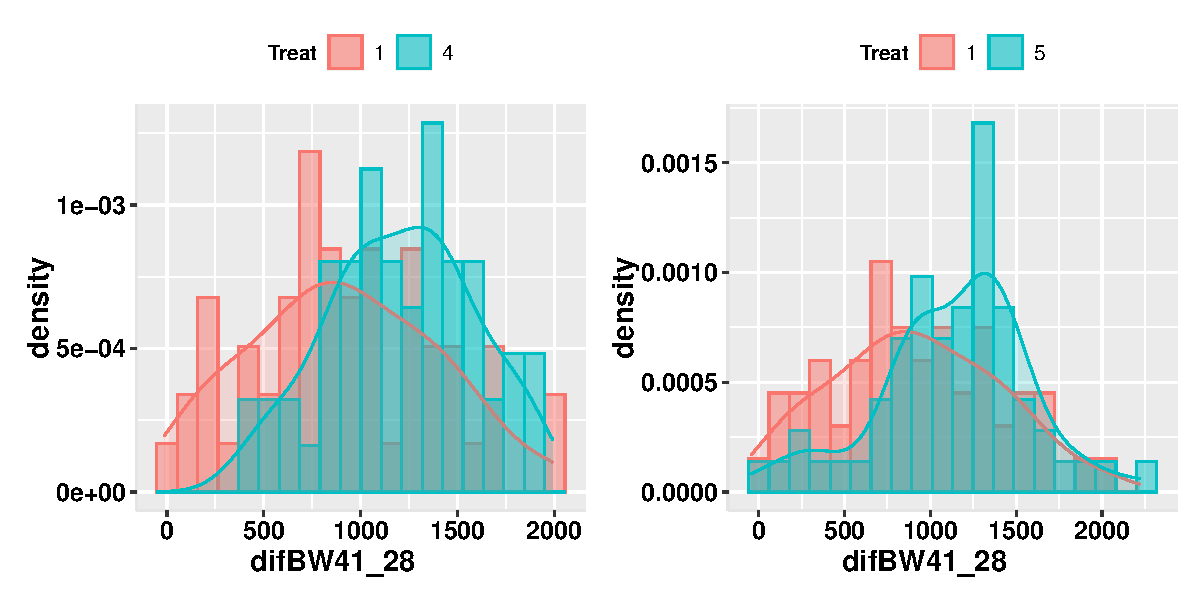
\includegraphics{def_files/figure-latex/unnamed-chunk-12-2.pdf}
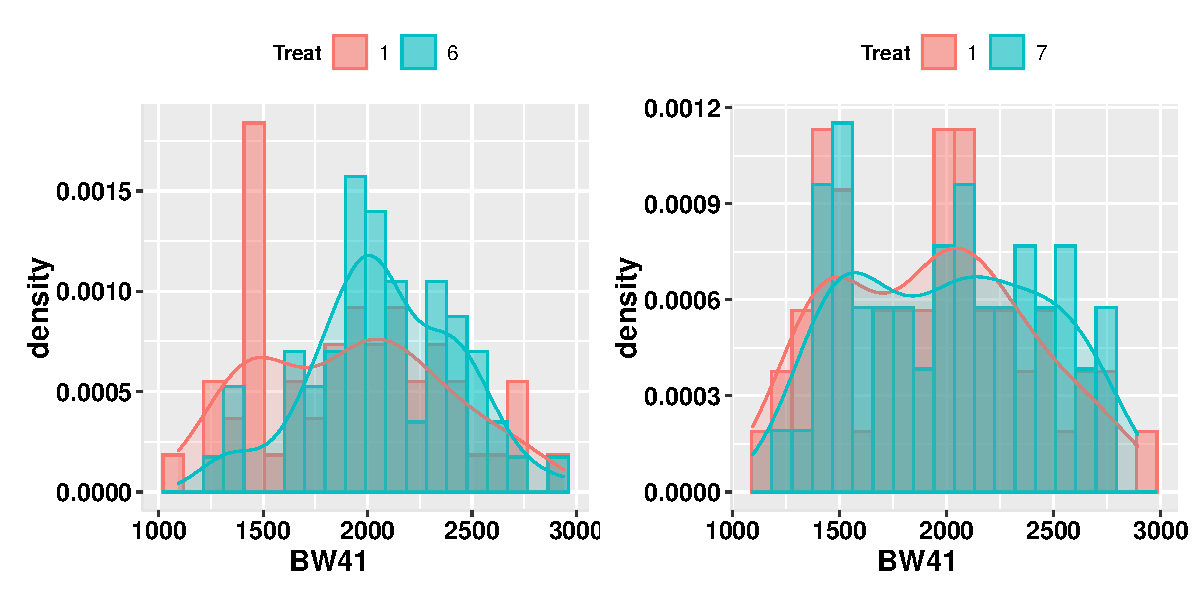
\includegraphics{def_files/figure-latex/unnamed-chunk-12-3.pdf}
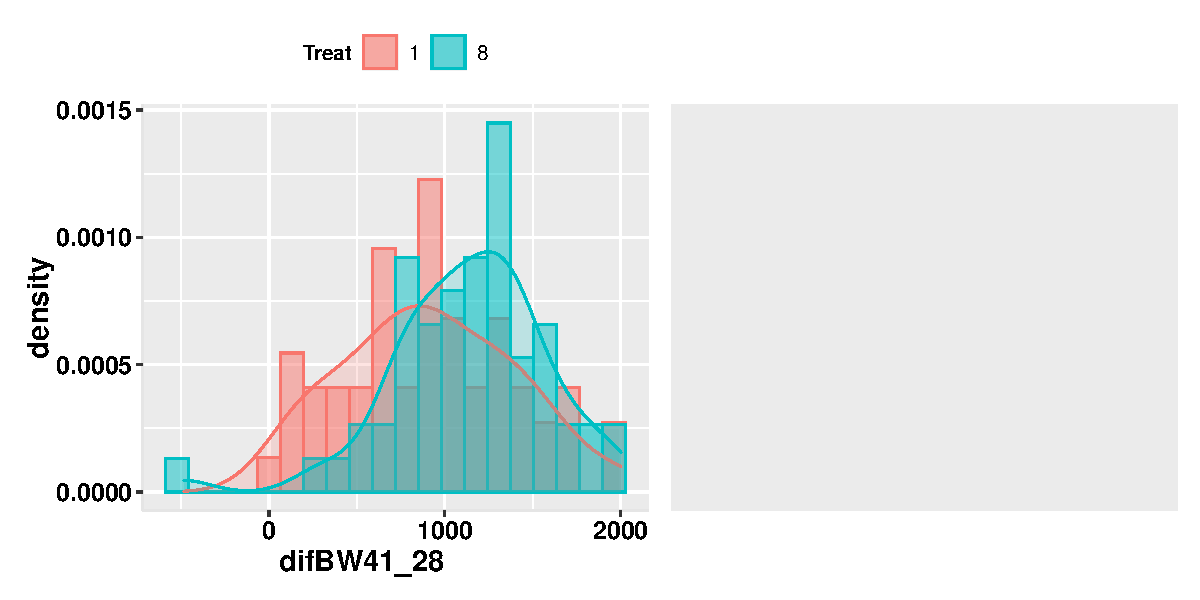
\includegraphics{def_files/figure-latex/unnamed-chunk-12-4.pdf}

\hypertarget{variable-difbw41_28}{%
\paragraph{\texorpdfstring{Variable
\emph{difBW41\_28}}{Variable difBW41\_28}}\label{variable-difbw41_28}}

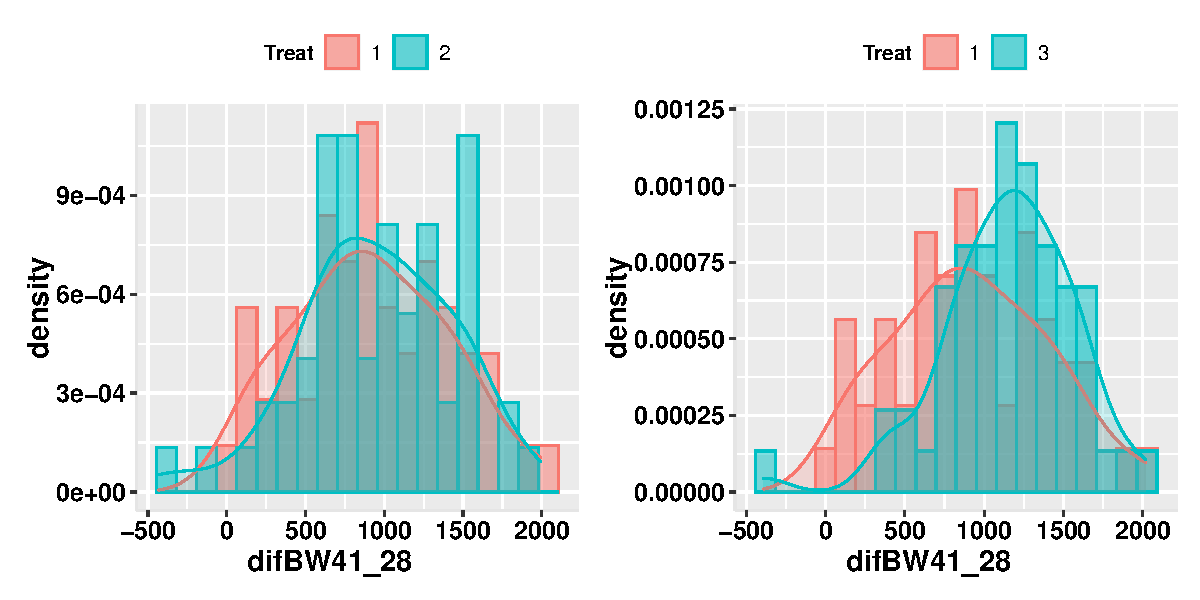
\includegraphics{def_files/figure-latex/unnamed-chunk-13-1.pdf}
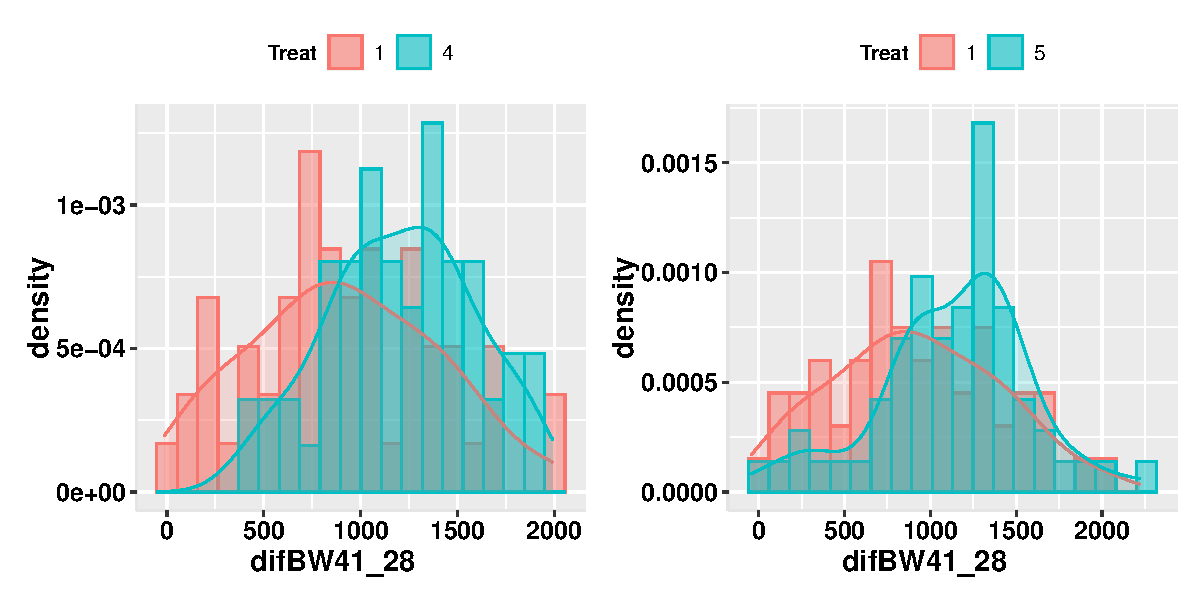
\includegraphics{def_files/figure-latex/unnamed-chunk-13-2.pdf}
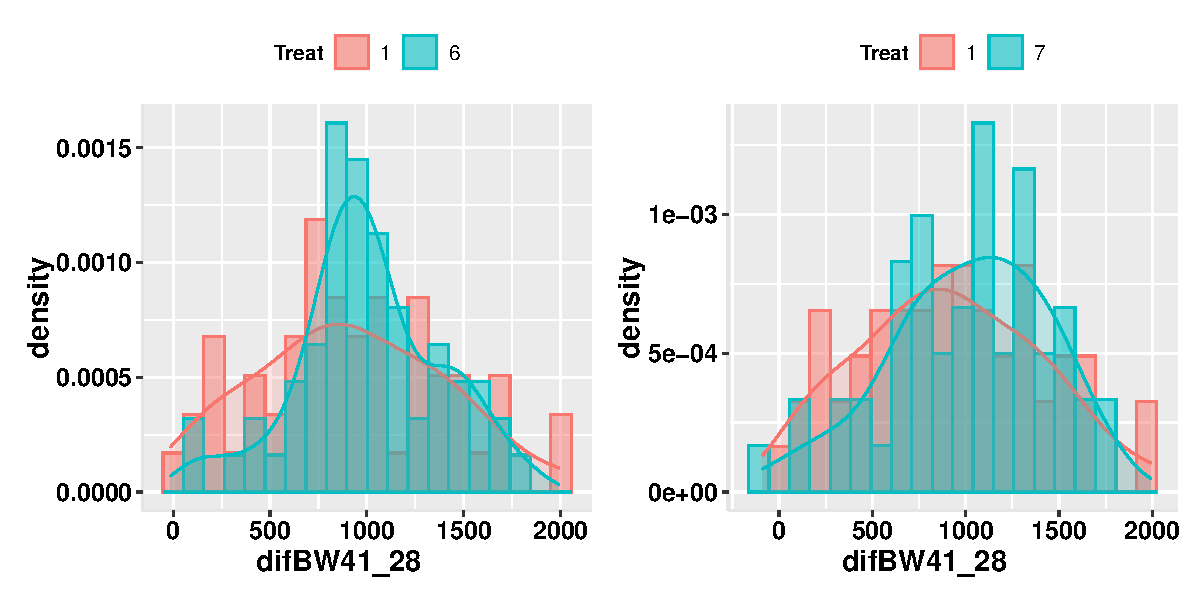
\includegraphics{def_files/figure-latex/unnamed-chunk-13-3.pdf}
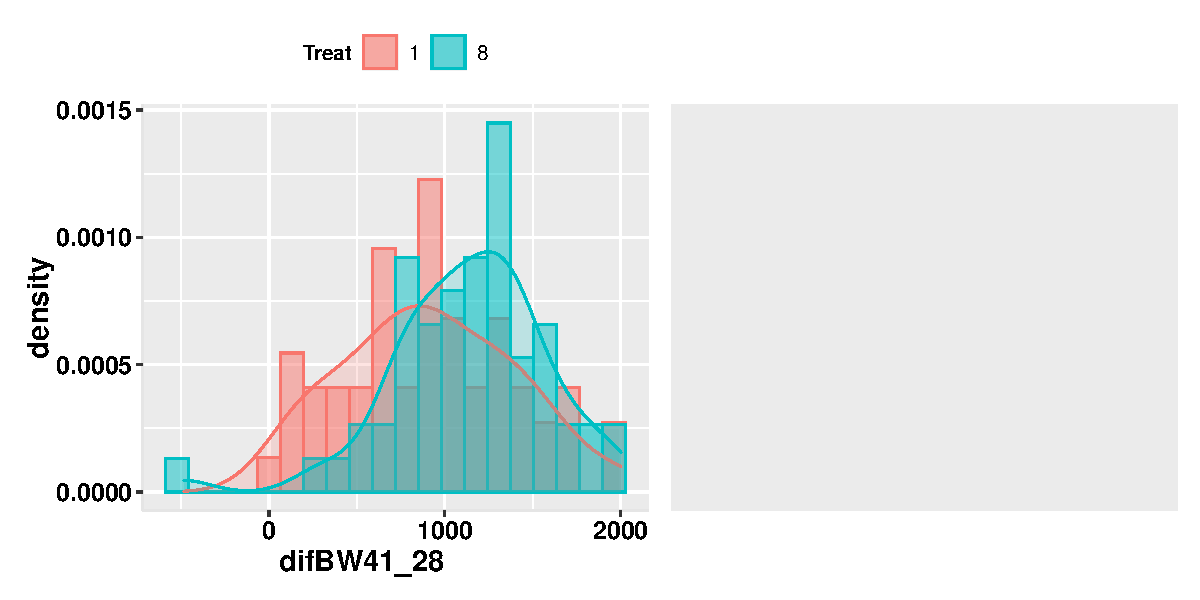
\includegraphics{def_files/figure-latex/unnamed-chunk-13-4.pdf}

\hypertarget{two-sample-rank-test-to-detect-a-shift-in-a-proportion-of-the-treated-population}{%
\subsubsection{Two-Sample Rank Test To Detect A Shift In A Proportion Of
The ``Treated''
Population}\label{two-sample-rank-test-to-detect-a-shift-in-a-proportion-of-the-treated-population}}

Test bi-mostral per detectar un canvi positiu en una proporció de la
població (tractament) comparada a una altra (control).

quantileTest(x, y, alternative = ``greater'', target.quantile = 0.5,
target.r = NULL, exact.p = TRUE)

\begin{itemize}
\item
  \(x\): Vector numèric d'observacions del grup tractament.
\item
  \(y\): Vector numèric d'observacions del grup control.
\item
  \(alternative\): Tipus d'hipòtesi alternativa.

  \begin{itemize}
  \item
    ``greater'': La cua dreta del grup tractament desplaçada cap a la
    dreta de la cua dreta del grup control.
  \item
    ``less'': La cua esquerra del grup tractament desplaçada cap a la
    esquerra de la cua esquerra del grup control.
  \end{itemize}
\item
  \(target.quantile\): Quantil utilitzat com a punt de tall inferior per
  a la prova. A causa de la naturalesa discreta dels quantils empírics,
  el límit superior dels possibles quantils empírics sovint difereix del
  valor de target.quantile.
\end{itemize}

\emph{\(H_1:\) La porció \(\epsilon\) de la distribució per al grup de
tractament (la distribució de X) es desplaça cap a la dreta de la
distribució per al grup de referència (la distribució de Y).}

\begin{verbatim}
## 
##  Quantile Test
## 
## data:  subset(pesInd, Treat == 2)$difBW41_28subset(pesInd, Treat == 1)$difBW41_28
## k (# x obs of r largest) = 94, r = 181, m = 115.00000, n = 111.00000,
## quantile.ub = 0.20264, p-value = 0.3206
## alternative hypothesis: true e is  0
\end{verbatim}

Tractaments Quantil 20 P-value quantileTest 1 1 503 0.320644315368672 2
2 573.8\\
3\\
4 1 503 0.00325007403022126 5 3 819\\
6\\
7 1 503 4.48868988689455e-05 8 4 883.6\\
9\\
10 1 503 9.09157381439041e-05 11 5 865.8\\
12\\
13 1 503 0.00555108064360543 14 6 745.2\\
15\\
16 1 503 0.295421547978408 17 7 609\\
18\\
19 1 503 0.0149908818313822 20 8 766\\
21

\hypertarget{skewness-i-kurtosi}{%
\subsection{Skewness i Kurtosi}\label{skewness-i-kurtosi}}

\begin{verbatim}
##            [,1]
## [1,] 1.01156635
## [2,] 0.14219864
## [3,] 0.02626804
## [4,] 2.85914072
## [5,] 0.48532589
## [6,] 0.46443755
## [7,] 0.19728038
## [8,] 0.48394297
\end{verbatim}

\begin{verbatim}
##            [,1]
## [1,]  1.7969308
## [2,]  0.2660273
## [3,]  1.2468064
## [4,] 15.6807456
## [5,]  0.9036873
## [6,]  0.1297607
## [7,] -0.2954785
## [8,]  0.9218744
\end{verbatim}

Observem que per la taxa de tots els tractaments existeix una skewness
positiva en major o menor mesura, és a dir una cua més llarga a la
dreta. Cal destacar que la taxa del tractament 3 podria considerarse
pràcticament simètrica.

En quant a la curtosi observem que tots els valors són prou propers a 3,
de manera que podrien considerarse mesocúrtiques i lleugerament
leptocúrtiques (amb pic i cues primes). Destaquen el tractament 4 molt
leptoicúrtic i el tractament 7 lleugerament platicúrtic.

\hypertarget{costos}{%
\subsection{Costos}\label{costos}}

Coste/kg PV (€/kg): La fórmula es: (coste pienso {[}€/kg{]} * consumo
pienso {[}kg{]}) / ganancia peso {[}kg{]}

\begin{verbatim}
##  [1] "Corral"                 "Treat"                  "Consum0-10 (kg)"       
##  [4] "Consum10-28(kg)"        "Consum28-41(kg)"        "BW0 (kg)"              
##  [7] "BW10 (kg)"              "BW28"                   "BW41"                  
## [10] "P. prod (\200/kg)"         "Dosi prod (kg/t)"       "P.STARt (\200/kg)"        
## [13] "P. GRO (\200/kg)"          "P. FIN(\200/kg)"           "Coste/kg PV (Starter)" 
## [16] "Coste/kg PV (Grower)"   "Coste/kg PV (Finisher)"
\end{verbatim}

\url{https://www.statisticssolutions.com/transforming-data-for-normality/}
\url{https://rcompanion.org/handbook/I_12.html}
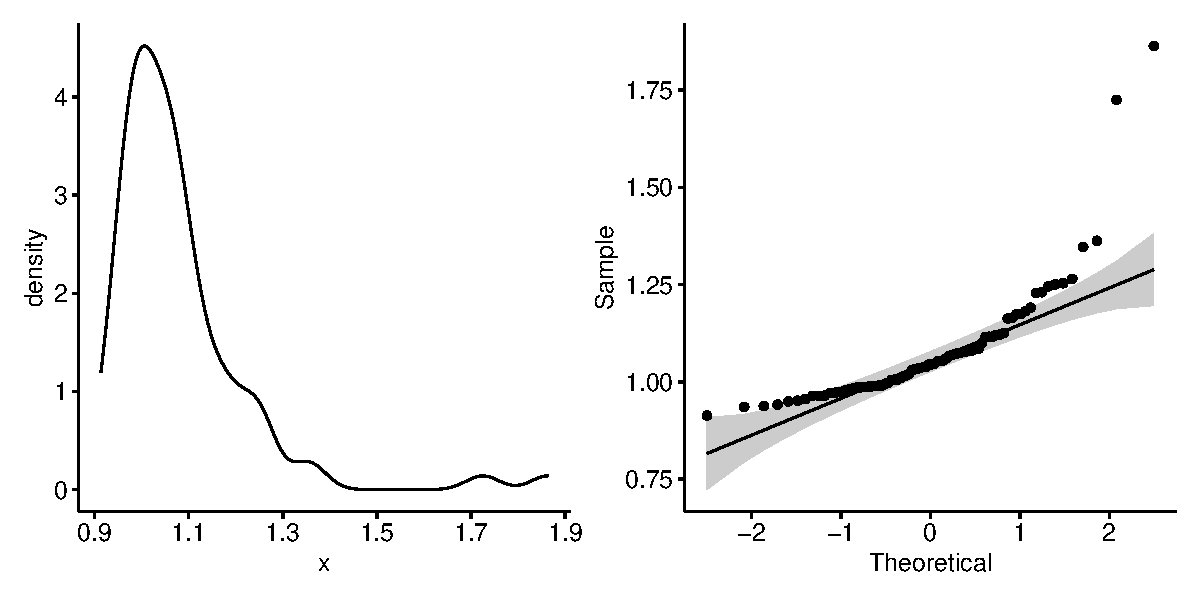
\includegraphics{def_files/figure-latex/unnamed-chunk-19-1.pdf}

\begin{verbatim}
## 
##  Shapiro-Wilk normality test
## 
## data:  c1
## W = 0.71771, p-value = 4.165e-11
\end{verbatim}

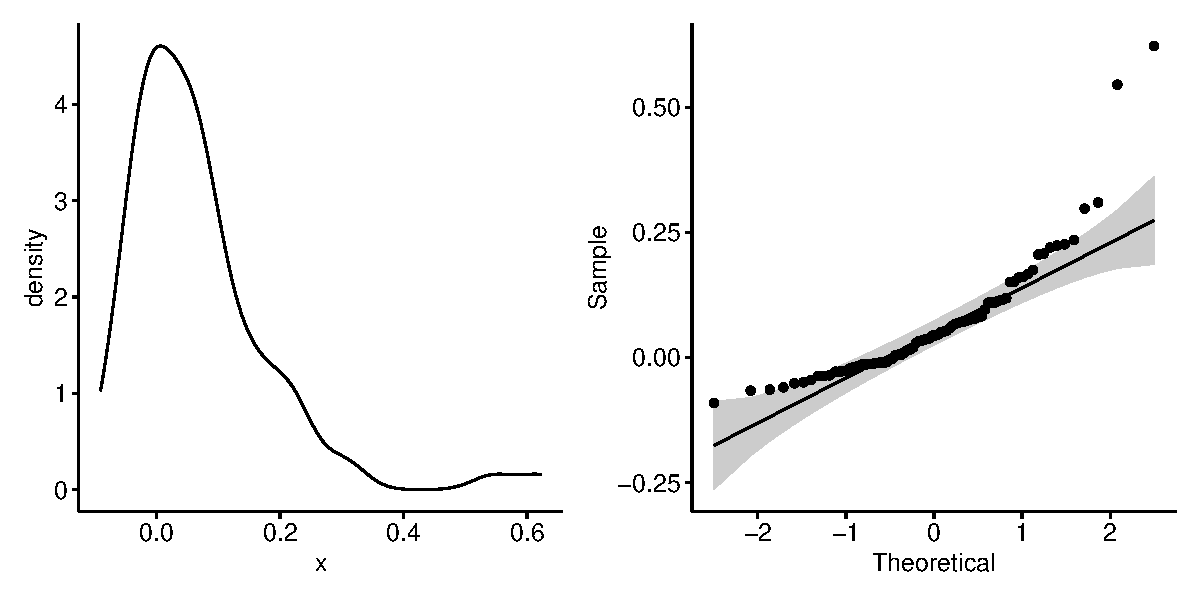
\includegraphics{def_files/figure-latex/unnamed-chunk-19-2.pdf}

\begin{verbatim}
## 
##  Shapiro-Wilk normality test
## 
## data:  c2
## W = 0.81113, p-value = 9.889e-09
\end{verbatim}

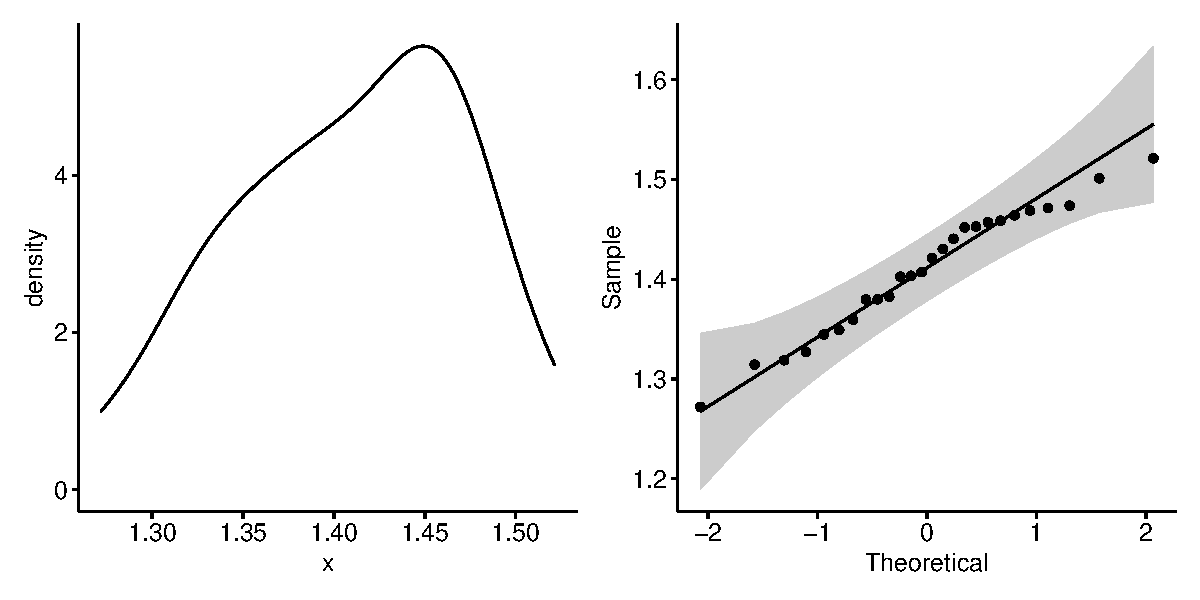
\includegraphics{def_files/figure-latex/unnamed-chunk-19-3.pdf}

\begin{verbatim}
## 
##  Shapiro-Wilk normality test
## 
## data:  c3
## W = 0.96936, p-value = 0.6069
\end{verbatim}

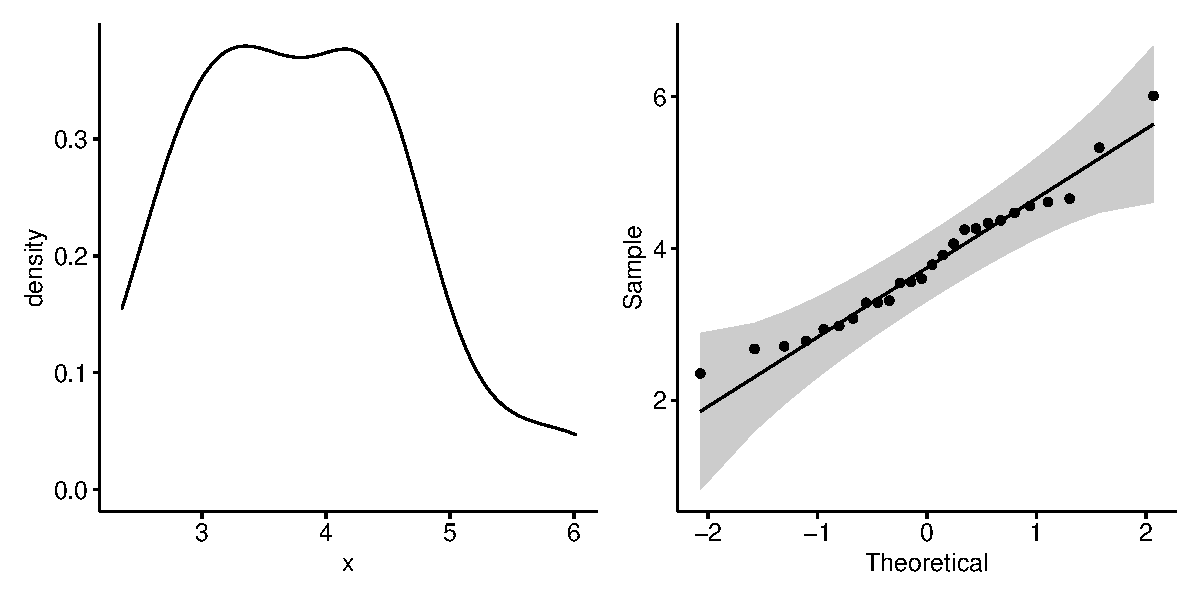
\includegraphics{def_files/figure-latex/unnamed-chunk-19-4.pdf}

\begin{verbatim}
## 
##  Shapiro-Wilk normality test
## 
## data:  c4
## W = 0.96606, p-value = 0.5245
\end{verbatim}

\begin{verbatim}
## 
##     lambda      W Shapiro.p.value
## 185   -5.4 0.9906          0.8288
## 
## if (lambda >  0){TRANS = x ^ lambda} 
## if (lambda == 0){TRANS = log(x)} 
## if (lambda <  0){TRANS = -1 * x ^ lambda}
\end{verbatim}

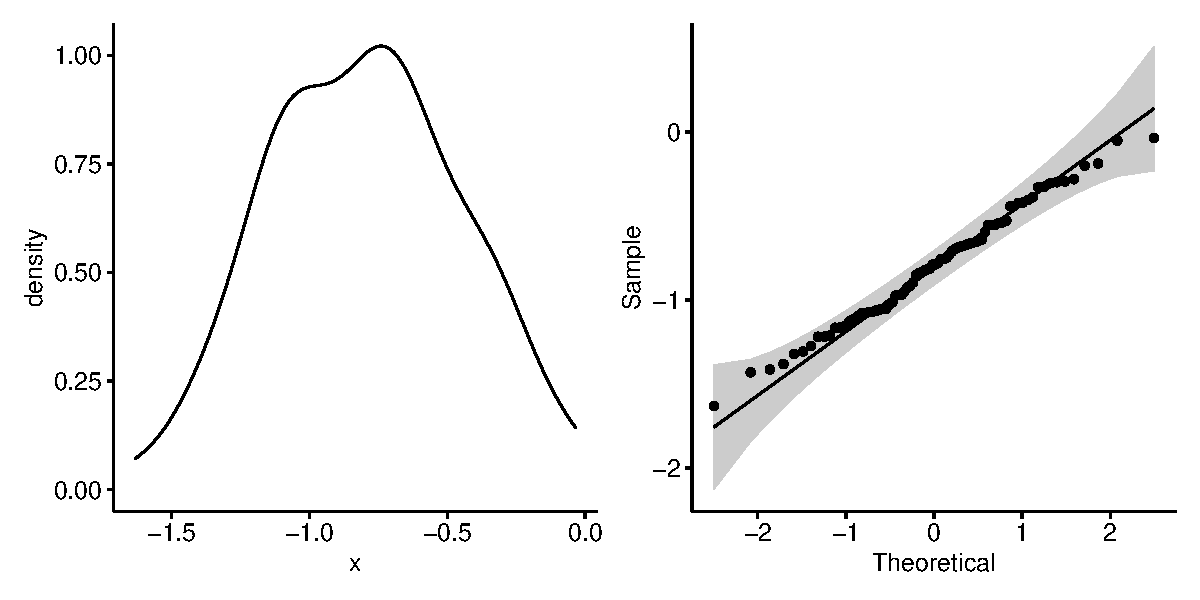
\includegraphics{def_files/figure-latex/unnamed-chunk-19-5.pdf}

\begin{verbatim}
## 
##  Shapiro-Wilk normality test
## 
## data:  c5
## W = 0.99055, p-value = 0.8288
\end{verbatim}

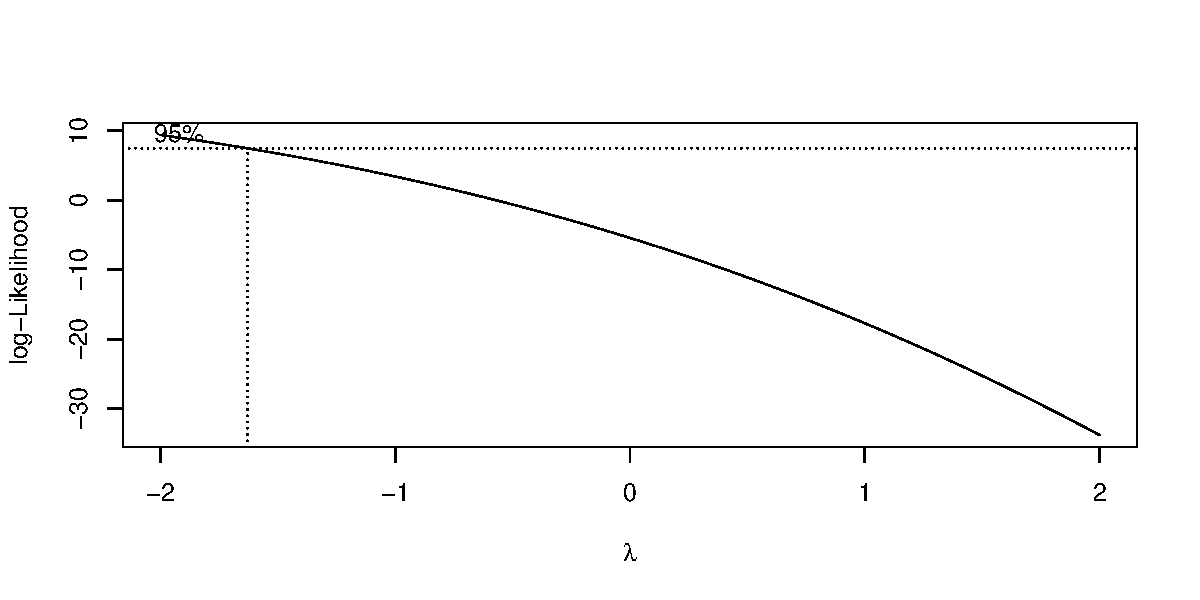
\includegraphics{def_files/figure-latex/unnamed-chunk-19-6.pdf}
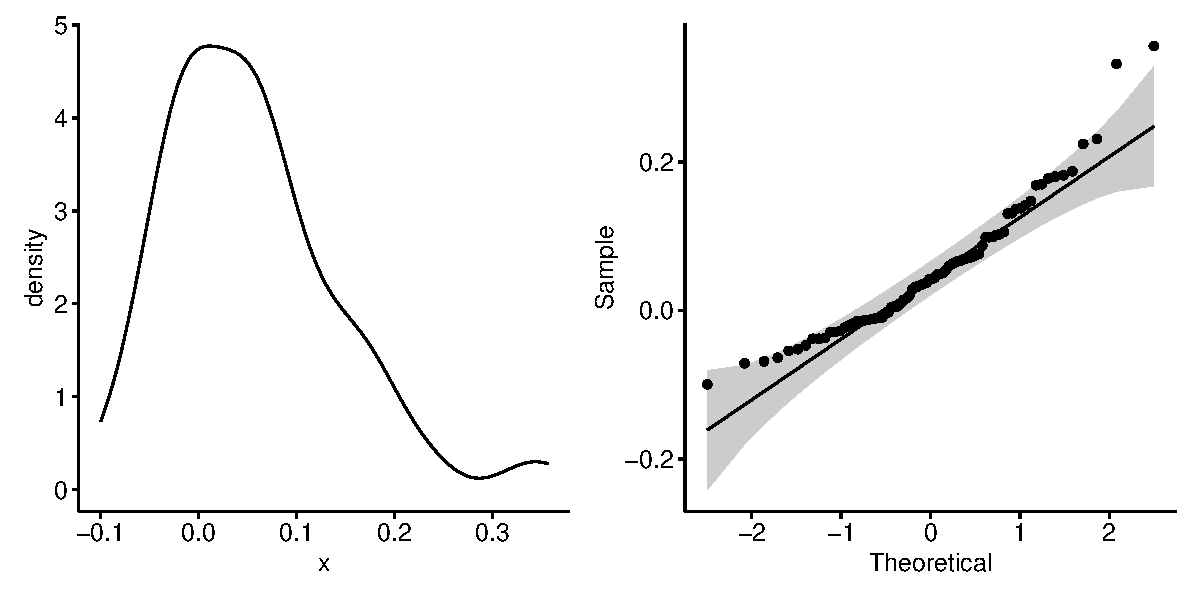
\includegraphics{def_files/figure-latex/unnamed-chunk-19-7.pdf}

\begin{verbatim}
## 
##  Shapiro-Wilk normality test
## 
## data:  c6
## W = 0.93468, p-value = 0.0005051
\end{verbatim}

\url{http://www.sthda.com/english/wiki/one-way-anova-test-in-r}

\begin{verbatim}
## tibble [80 x 4] (S3: tbl_df/tbl/data.frame)
##  $ Cost   : num [1:80] 1.07 1.73 1.16 1.07 1.07 ...
##  $ Box    : Factor w/ 80 levels "1","2","3","4",..: 1 11 18 26 34 41 50 60 65 75 ...
##  $ Treat  : Factor w/ 8 levels "1","2","3","4",..: 1 1 1 1 1 1 1 1 1 1 ...
##  $ CostTuk: num [1:80] -0.682 -0.0526 -0.4406 -0.7103 -0.689 ...
\end{verbatim}

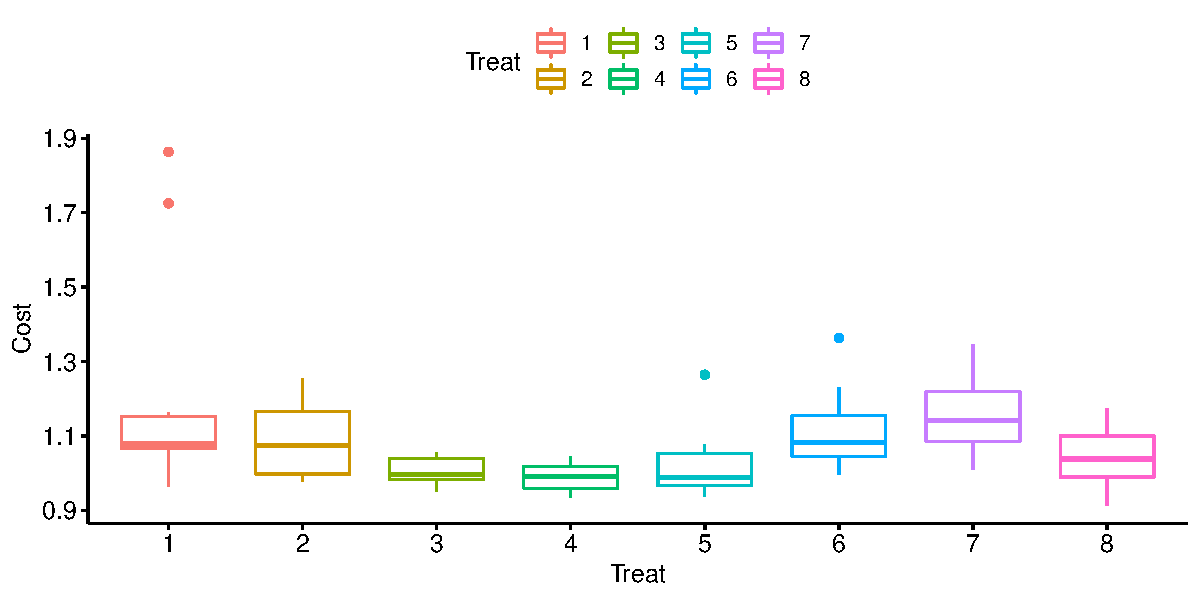
\includegraphics{def_files/figure-latex/unnamed-chunk-21-1.pdf}
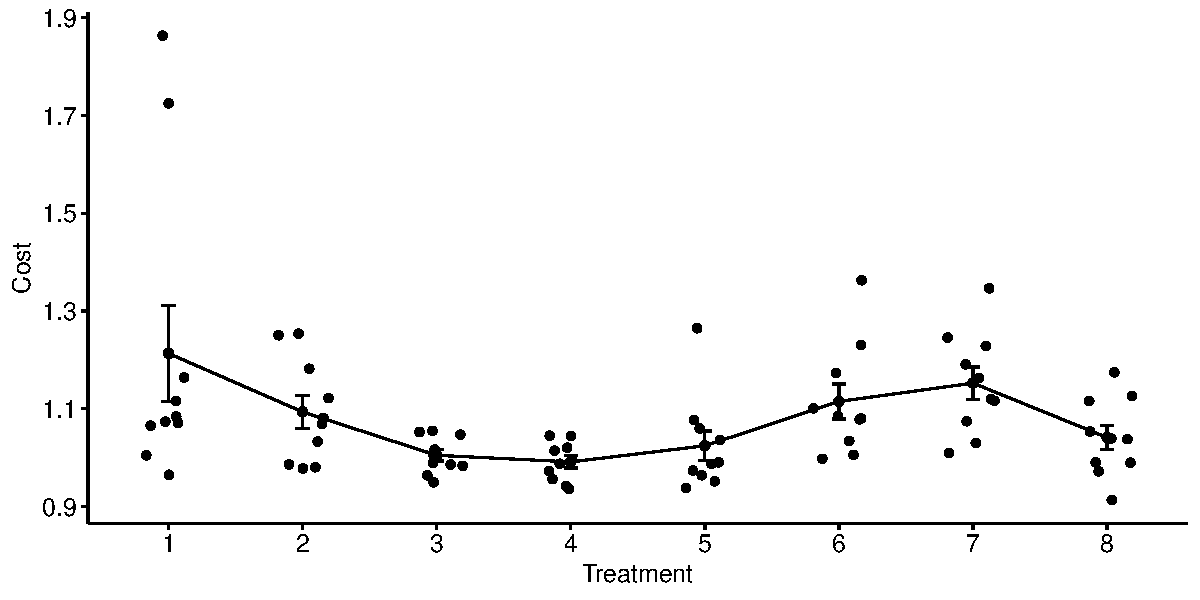
\includegraphics{def_files/figure-latex/unnamed-chunk-21-2.pdf}

\begin{verbatim}
##             Df Sum Sq Mean Sq F value   Pr(>F)    
## Treat        7  3.035  0.4336   4.881 0.000152 ***
## Residuals   72  6.397  0.0888                     
## ---
## Signif. codes:  0 '***' 0.001 '**' 0.01 '*' 0.05 '.' 0.1 ' ' 1
\end{verbatim}

Tukey multiple pairwise-comparisons

\begin{verbatim}
##   Tukey multiple comparisons of means
##     95% family-wise confidence level
## 
## Fit: aov(formula = CostTuk ~ Treat, data = costos)
## 
## $Treat
##            diff         lwr         upr     p adj
## 2-1 -0.10534095 -0.52147417  0.31079227 0.9931367
## 3-1 -0.39553259 -0.81166581  0.02060063 0.0743188
## 4-1 -0.47522197 -0.89135519 -0.05908875 0.0142789
## 5-1 -0.37332879 -0.78946201  0.04280442 0.1109716
## 6-1 -0.03179923 -0.44793244  0.38433399 0.9999976
## 7-1  0.07552814 -0.34060507  0.49166136 0.9991567
## 8-1 -0.27980476 -0.69593797  0.13632846 0.4254439
## 3-2 -0.29019164 -0.70632486  0.12594157 0.3777193
## 4-2 -0.36988102 -0.78601424  0.04625220 0.1177964
## 5-2 -0.26798785 -0.68412106  0.14814537 0.4823023
## 6-2  0.07354172 -0.34259150  0.48967494 0.9992911
## 7-2  0.18086909 -0.23526413  0.59700231 0.8732801
## 8-2 -0.17446381 -0.59059703  0.24166941 0.8926083
## 4-3 -0.07968937 -0.49582259  0.33644384 0.9988066
## 5-3  0.02220380 -0.39392942  0.43833702 0.9999998
## 6-3  0.36373337 -0.05239985  0.77986658 0.1307916
## 7-3  0.47106074  0.05492752  0.88719396 0.0156775
## 8-3  0.11572784 -0.30040538  0.53186105 0.9879685
## 5-4  0.10189317 -0.31424005  0.51802639 0.9943951
## 6-4  0.44342274  0.02728952  0.85955596 0.0286039
## 7-4  0.55075011  0.13461689  0.96688333 0.0023292
## 8-4  0.19541721 -0.22071601  0.61155043 0.8225572
## 6-5  0.34152957 -0.07460365  0.75766279 0.1871716
## 7-5  0.44885694  0.03272372  0.86499016 0.0254839
## 8-5  0.09352404 -0.32260918  0.50965726 0.9967007
## 7-6  0.10732737 -0.30880585  0.52346059 0.9923168
## 8-6 -0.24800553 -0.66413875  0.16812769 0.5818409
## 8-7 -0.35533290 -0.77146612  0.06080032 0.1503343
\end{verbatim}

\begin{verbatim}
##            diff        lwr         upr      p adj
## 2-1 -0.10534095 -0.5214742  0.31079227 0.99313670
## 3-1 -0.39553259 -0.8116658  0.02060063 0.07431879
## 4-1 -0.47522197 -0.8913552 -0.05908875 0.01427889
## 5-1 -0.37332879 -0.7894620  0.04280442 0.11097158
## 6-1 -0.03179923 -0.4479324  0.38433399 0.99999757
## 7-1  0.07552814 -0.3406051  0.49166136 0.99915669
## 8-1 -0.27980476 -0.6959380  0.13632846 0.42544395
\end{verbatim}

Multiple comparisons using multcomp package

\begin{verbatim}
## [1] "summary.glht" "glht"
\end{verbatim}

\begin{verbatim}
##  [1] "model"       "linfct"      "rhs"         "coef"        "vcov"       
##  [6] "df"          "alternative" "type"        "focus"       "test"
\end{verbatim}

Pairewise t-test

\begin{verbatim}
## 
##  Pairwise comparisons using t tests with pooled SD 
## 
## data:  costos$CostTuk and costos$Treat 
## 
##   1      2      3      4      5      6      7     
## 2 0.5691 -      -      -      -      -      -     
## 3 0.0190 0.0764 -      -      -      -      -     
## 4 0.0067 0.0246 0.6277 -      -      -      -     
## 5 0.0246 0.0963 0.8682 0.5691 -      -      -     
## 6 0.8422 0.6277 0.0248 0.0078 0.0318 -      -     
## 7 0.6277 0.2949 0.0067 0.0027 0.0078 0.5691 -     
## 8 0.0847 0.3030 0.5691 0.2572 0.5907 0.1249 0.0265
## 
## P value adjustment method: BH
\end{verbatim}

Check ANOVA assumptions: test validity?

Check the homogeneity of variance assumption
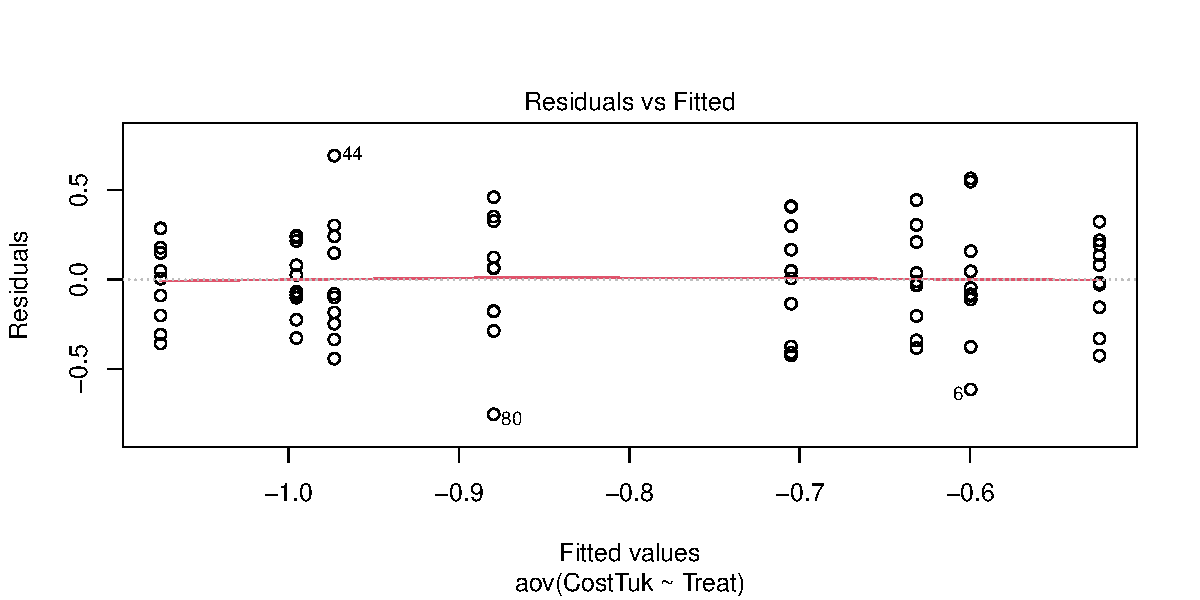
\includegraphics{def_files/figure-latex/unnamed-chunk-25-1.pdf}

\begin{verbatim}
## Levene's Test for Homogeneity of Variance (center = median)
##       Df F value Pr(>F)
## group  7  0.5332 0.8066
##       72
\end{verbatim}

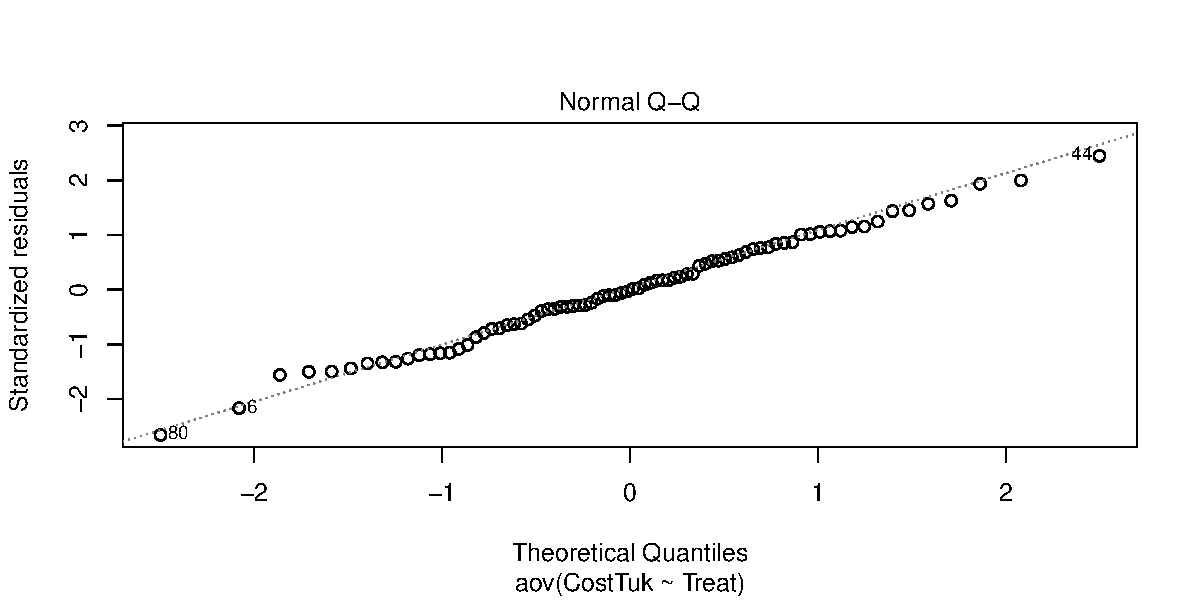
\includegraphics{def_files/figure-latex/unnamed-chunk-27-1.pdf}

\begin{verbatim}
## 
##  Shapiro-Wilk normality test
## 
## data:  residuals(anova)
## W = 0.99411, p-value = 0.9764
\end{verbatim}

Non-parametric alternative to one-way ANOVA test

\begin{verbatim}
## 
##  Kruskal-Wallis rank sum test
## 
## data:  CostTuk by Treat
## Kruskal-Wallis chi-squared = 26.31, df = 7, p-value = 0.0004432
\end{verbatim}

\end{document}
